
\chapter{Geodesia}


\section{Definiciones básicas}

Como sabemos la tierra tiene una forma de una esfera achatada, tomando la forma de un elipsoide de revolución. En palabras de Isaac Newton: <<Una forma de equilibrio que tiene una masa bajo el influjo de las leyes de gravitación y girando en torno a su eje es la de un esferoide aplastado en sus polos>>. Un \textit{esferoide aplastado en sus polos} es básicamente un elipsoide de revolución. Definimos pues:



\begin{itemize}
	\begin{minipage}{.45\textwidth}
	\item   \textbf{Polos:} puntos de corte entre el eje menor de la elipse y elipsoide. Llamamos polo norte (PN) al corte superior y polo sur (PS) al corte superior.   
	\item \textbf{Ecuador terrestre:} línea circular correspondiente al corte entre el plano perpendicular al eje menor que pasa por el centro del elipsoide y este.
	\end{minipage}	\hfill
	\begin{minipage}{0.45\textwidth} \centering
	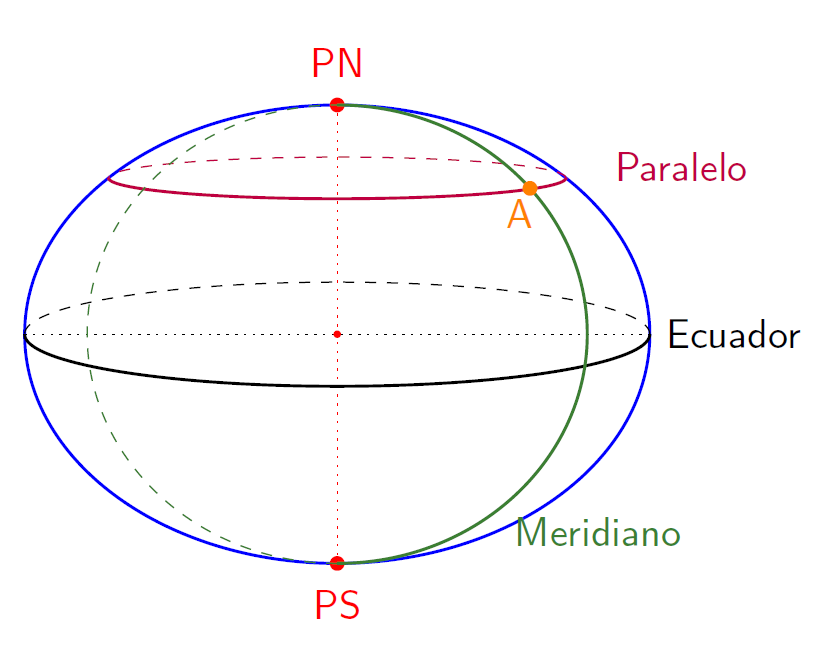
\includegraphics[scale=0.37]{Cuerpo/Imagenes/01_Elipsoide.png} 
	\end{minipage}
\end{itemize}
\begin{itemize}
	\item \textbf{Paralelos:} líneas circulares correspondientes a los cortes entre los planos paralelos al ecuador (paralelo cero) y el elipsoide.
	\item \textbf{Meridianos:} líneas elipsoidales determinadas por el corte entre el elipsoide y el hazde planos que define el eje menor. Se considera \textit{meridiano cero} al que pasa por Greenwich.
	\item \textbf{Vertical de lugar:} es la línea normal al elipsoide en un punto dado.
\end{itemize}


Al conjunto de variables que permiten describir cualquier punto de la Tierra se le llaman \textit{coordenadas terrestres}, y existen dos tipos de coordenadas terrestres, que se definen en función de la \textit{vertical de lugar}

\begin{itemize}
	\item \textbf{Coordenadas geográficas:} son dos variables angulares ($\phi,\lambda$), que se definen como

	\begin{itemize}	
		\item \textbf{Latitud geográfica} $\phi$. Toma valores de $90^\circ$ a $-90^\circ$. Para un punto $A$ cualquiera el ángulo $\phi$ es el comprendido entre la vertical de lugar y el ecuador.
		\item \textbf{Longitud geográfica} $\lambda$. Toma valores entre $180^\circ$ y $-180^\circ$. Para un punto $A$ cualquiera el ángulo $\lambda$ se define como aquel entre la vertical de lugar y el meridiano de Greenwich. 
	\end{itemize}
	
	\item \textbf{Coordenadas geocéntricas}: consta de tres variables $(\rho,\psi,\lambda)$, dos angulares y una distancia. Estas son: 
	
	\vspace{2mm}
		
	\begin{minipage}{1\textwidth}
	 \begin{itemize}
	\item \textbf{Radio vector} $\rho$. Distancia entre el centro de la tierra (punto 0) y el punto A. 
	\end{itemize}
	\end{minipage}	

	\begin{minipage}{.5\textwidth}
	\begin{itemize}
		\item \textbf{Latitud geocéntrica} $\psi$. Toma valores de $90^\circ$ a $-90^\circ$. Para un punto $A$ cualquiera el ángulo $\psi$ es el comprendido entre el radio y el ecuador. 
		\item \textbf{Longitud geocéntrica} $\lambda$. Se define igual que la longitud geográfica. Toma valores entre $180^\circ$ y $-180^\circ$. Para un punto $A$ cualquiera el ángulo $\lambda$ se define como aquel entre la vertical de lugar y el meridiano de Greenwich.
	\end{itemize}
	\end{minipage}	\hfill
	\begin{minipage}{0.5\textwidth} \centering
		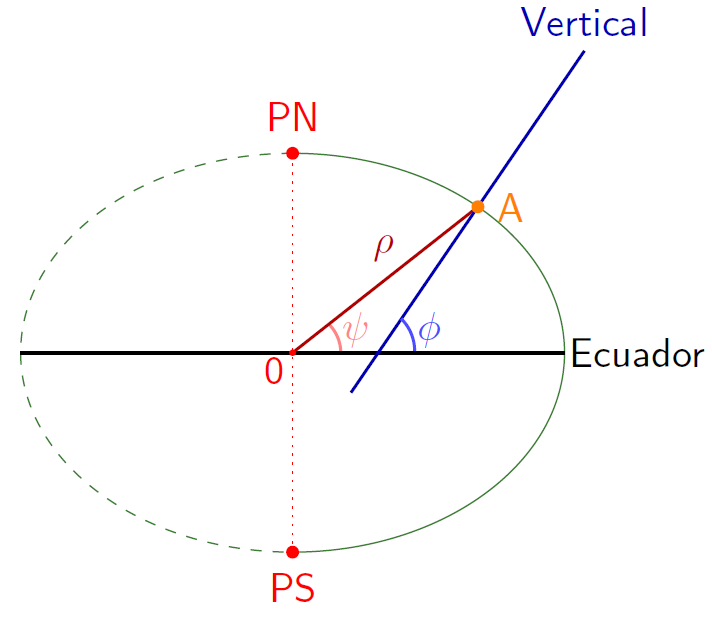
\includegraphics[scale=0.42]{Cuerpo/Imagenes/01_Coordenadas.png} 
	\end{minipage}	
	
\end{itemize}

Otra definición importante es la del \textbf{plano del horizonte}, que es el plano perpendicular a la vertical de lugar en el punto $A$. El plano horizonte pertenece a la llamada \textbf{esfera celeste topocéntrica}, que es aquella cuyo centro es el observador. En esta esfera, el plano horizonte define lo que una persona diría que es arriba y abajo. La esfera celeste tropocéntrica tiene también un polo norte celeste (PNC) y un polo sur celeste (PSC) paralelo con el eje del mundo, pero no necesariamente con el <<arriba>> del observador. Al punto $Z$ se le llama \textbf{cénit} y al punto $Z'$ se le llama \textbf{nádir}.

\begin{figure}[h]
	\centering
	\begin{subfigure}{0.55\textwidth}
		\centering
		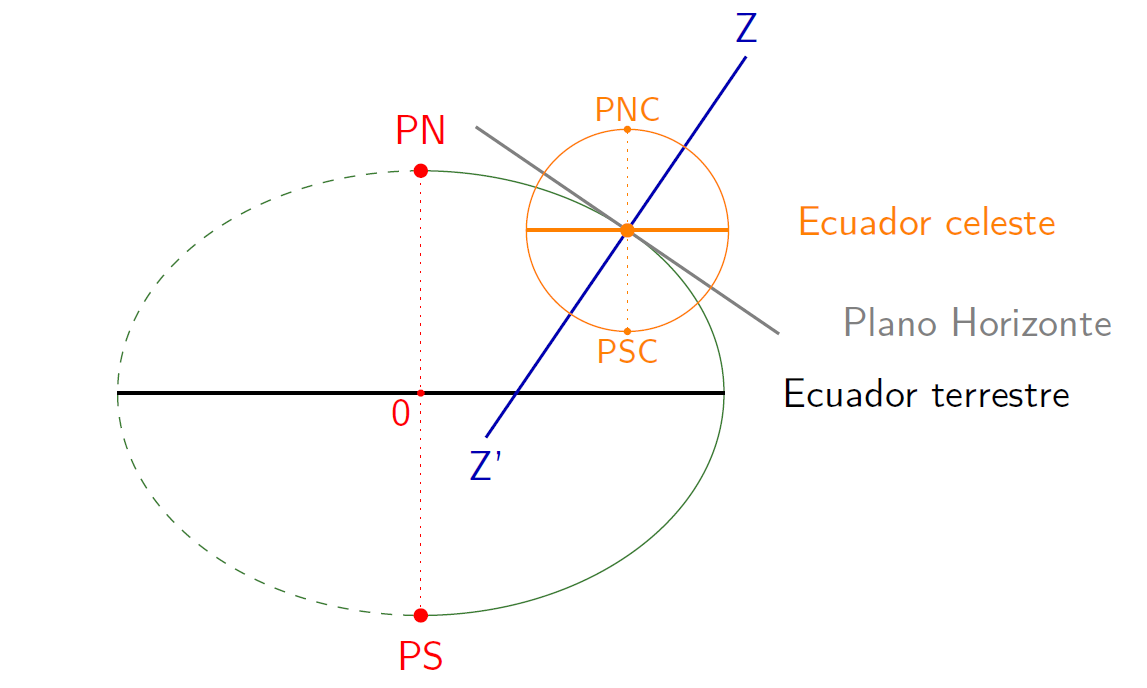
\includegraphics[width=1\textwidth]{Cuerpo/Imagenes/01_Plano.png}
	\end{subfigure}
	\hfill
	\begin{subfigure}{0.4\textwidth}
		\centering
		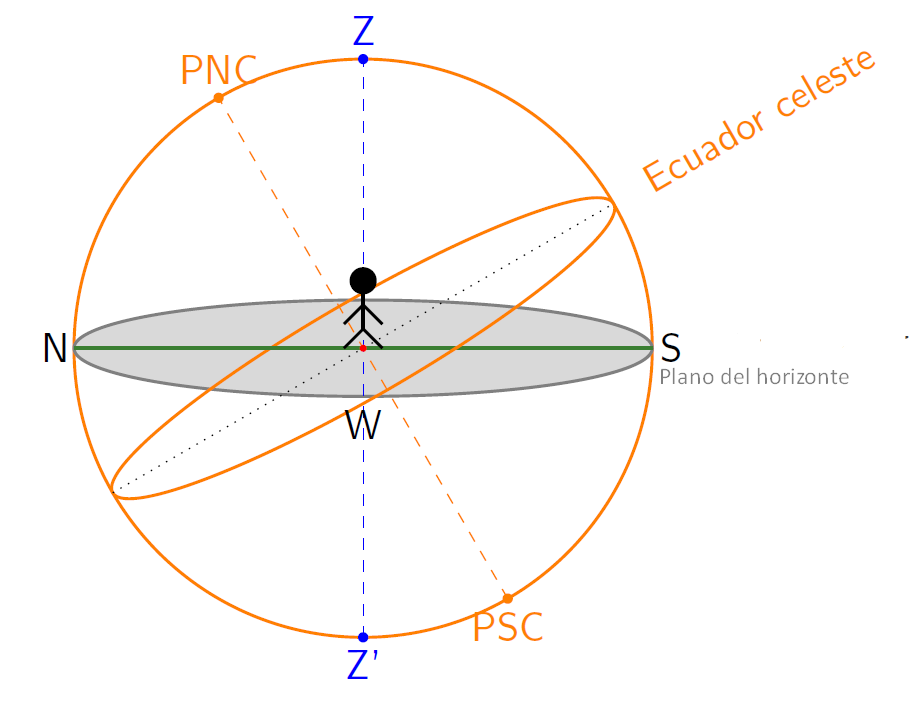
\includegraphics[width=1\textwidth]{Cuerpo/Imagenes/01_Esfera.png}
	\end{subfigure}
\end{figure}
Como podemos ver el ángulo entre la línea PNC y Z en la esfera topocéntrica es igual a $90^\circ - \phi$, y por tanto independiente al meridiano en el que nos encontremos, solo depende del paralelo en el que se encuentre el punto del observador. A dicho ángulo se le llama \textbf{colatitud}.


\section{Coordenadas celestes}

\begin{Anotacion}
	\textcolor{red}{Aquí tenemos que hablar de las coordenadas horizontales y horarias de la esfera celeste. Para que sirven cada una, como se definen. Relaciones entre ellas.}
\end{Anotacion}	

% Las coordenadas horizontales constituyen un sistema de coordenadas local, mientras que las coordenadas ecuatoriales horarias constituyen uno semilocal.


El \textbf{plano de la eclíptica} es el plano que contiene la órbita de la Tierra alrededor del Sol, y está inclinado con respecto al ecuador celeste una cantidad llamada \textit{oblicuidad de la eclíptica} $\varepsilon=20^\circ 26'29''$. En la esfera celeste geocéntrica, cuyo centro es la Tierra, es el Sol quien aparenta moverse a nuestro alrededor. Llamamos \textbf{eclíptica} a la intersección del plano de la eclíptica con la esfera celesta.

\begin{figure}[h]
	\centering
	\begin{subfigure}{0.45\textwidth}
		\centering
		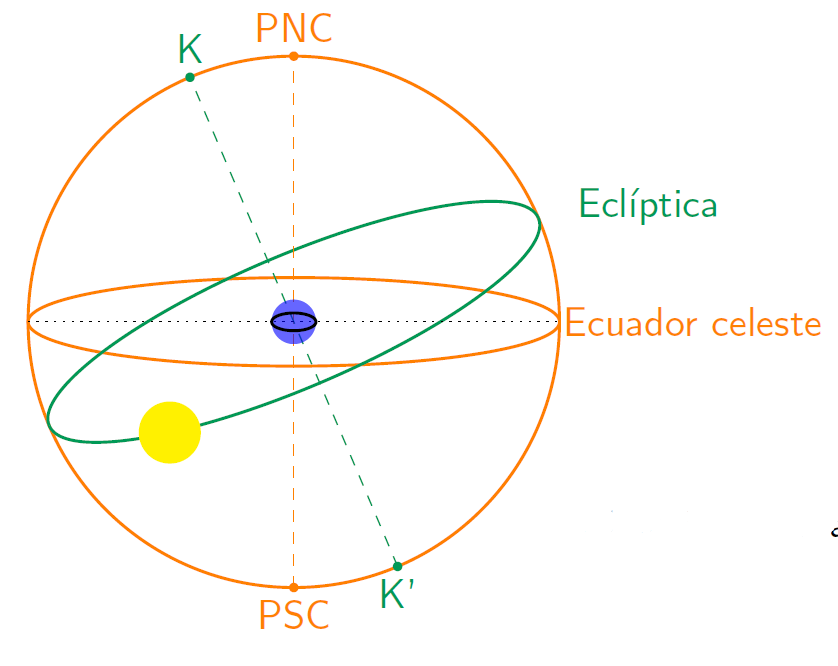
\includegraphics[width=1\textwidth]{Cuerpo/Imagenes/01_Ecliptica.png}
	\end{subfigure}
	\hfill
	\begin{subfigure}{0.45\textwidth}
		\centering
		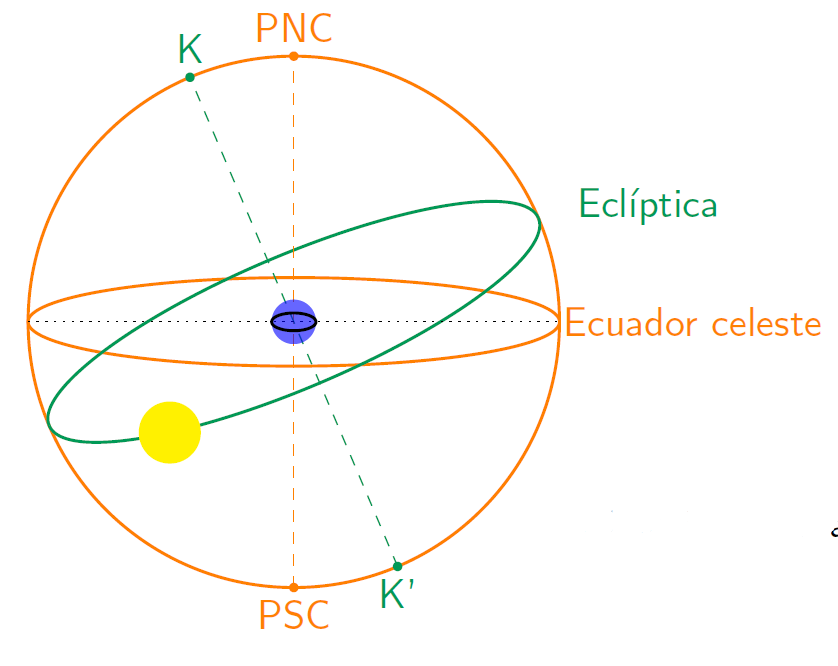
\includegraphics[width=1\textwidth]{Cuerpo/Imagenes/01_Ecliptica.png}
	\end{subfigure}
\end{figure}




\begin{Anotacion}
	\textcolor{red}{Esfera celeste, en este orden: coordenadas eclípticas, horizontales, absolutas. Para que sirve cada uno, cuales son los ángulos de referencia. En las ecuatoriales hay que hablar de los ángulos del equinocio y solscitio del sol. En lass horizontales también. Como se cambia de un sistema de coordenadas a otra. Matrices de rotación. Tiempo sideral. Diferencia entre levógiro y dextrógiro. }
\end{Anotacion}	

%Las coordenadas celestes ecuatoriales absolutas y eclípticas constituyen sistemas de coordenadas absolutos, siendo independientes de los movimientos de rotación y traslación de la Tierra. Sin embargo, existen otros movimientos de la Tierra que sí afectan a las coordenadas. Veremos los movimietnos de precesión y nutación. 

\section{Ejercicios}


\tcbstartrecording
\begin{texercise}
	
	Prueba que el azimut y el ángulo horario de un astro en sus puntos de orto y ocaso, $A_0$ y $H_0$, para un observador a una latitud $\phi$, satisfacen la siguientes relaciones:
	
	\begin{equation}
		\cos (A_0) = - \frac{\sin (\delta)}{\cos (\phi)} \tquad \cos (H_0) = - \tan \delta \tan \phi
	\end{equation}
	\tcblower

	Recordamos que el orto y ocaso son los lugares del plano horizonte donde empieza a ser visible y deja de ser visible. Con respecto las coordenadas horizontales, la altura es cero $h=0^\circ$, o lo que es lo mismo $z=90^\circ$. Ahora tenemos que usar las coordenadas de Bessel, que relaciona las coordenadas horizonatles (A,h) y horarias ($H,\delta$):
	
	\begin{equation}
	\begin{pmatrix}
		\cos \delta \cos H \\
		\cos \delta \sin H \\
		\sin \delta 
	\end{pmatrix} =\begin{pmatrix}
		\sin \phi & 0 & \cos \phi \\
		0 & 1 & 0 \\
		- \cos \phi & 0 & \sin \phi
	\end{pmatrix}
	\begin{pmatrix}
		\cos h \cos A \\
		\cos h \sin A \\
		\sin h
	\end{pmatrix}
	\end{equation}
	de lo cual se deduce que
	
	\begin{equation}
	\sin \delta = - \cos (\phi) \cos A_0  \Rightarrow \cos (A_0) = - \frac{\sin \delta}{\cos \phi}
	\end{equation}
	Y también se deduce que
	
	\begin{equation}
	\cos \delta \cos H_0 = \sin \phi \cos A_0 \Rightarrow \cos (H_0) = \frac{\sin \phi}{\cos \delta} \parentesis{ - \frac{\sin \delta}{\cos \phi}} \Rightarrow \cos (H_0) = - \tan \delta \tan \phi
	\end{equation}
\end{texercise}

\begin{texercise}
	 ¿Cómo relacionarías la información proporcionada por $H_0$ con el tiempo que un astro permanece por encima del horizonte?
	 \tcblower
	 
	 \begin{minipage}{.45\textwidth} 	
	 	El tiempo que un astro está encima del horizonte corresponde a $2H_0$. Puso $H_{\text{orto}}=-H_{\text{ocaso}}$.
	 \end{minipage}	\hfill
	 \begin{minipage}{0.45\textwidth} 
	 	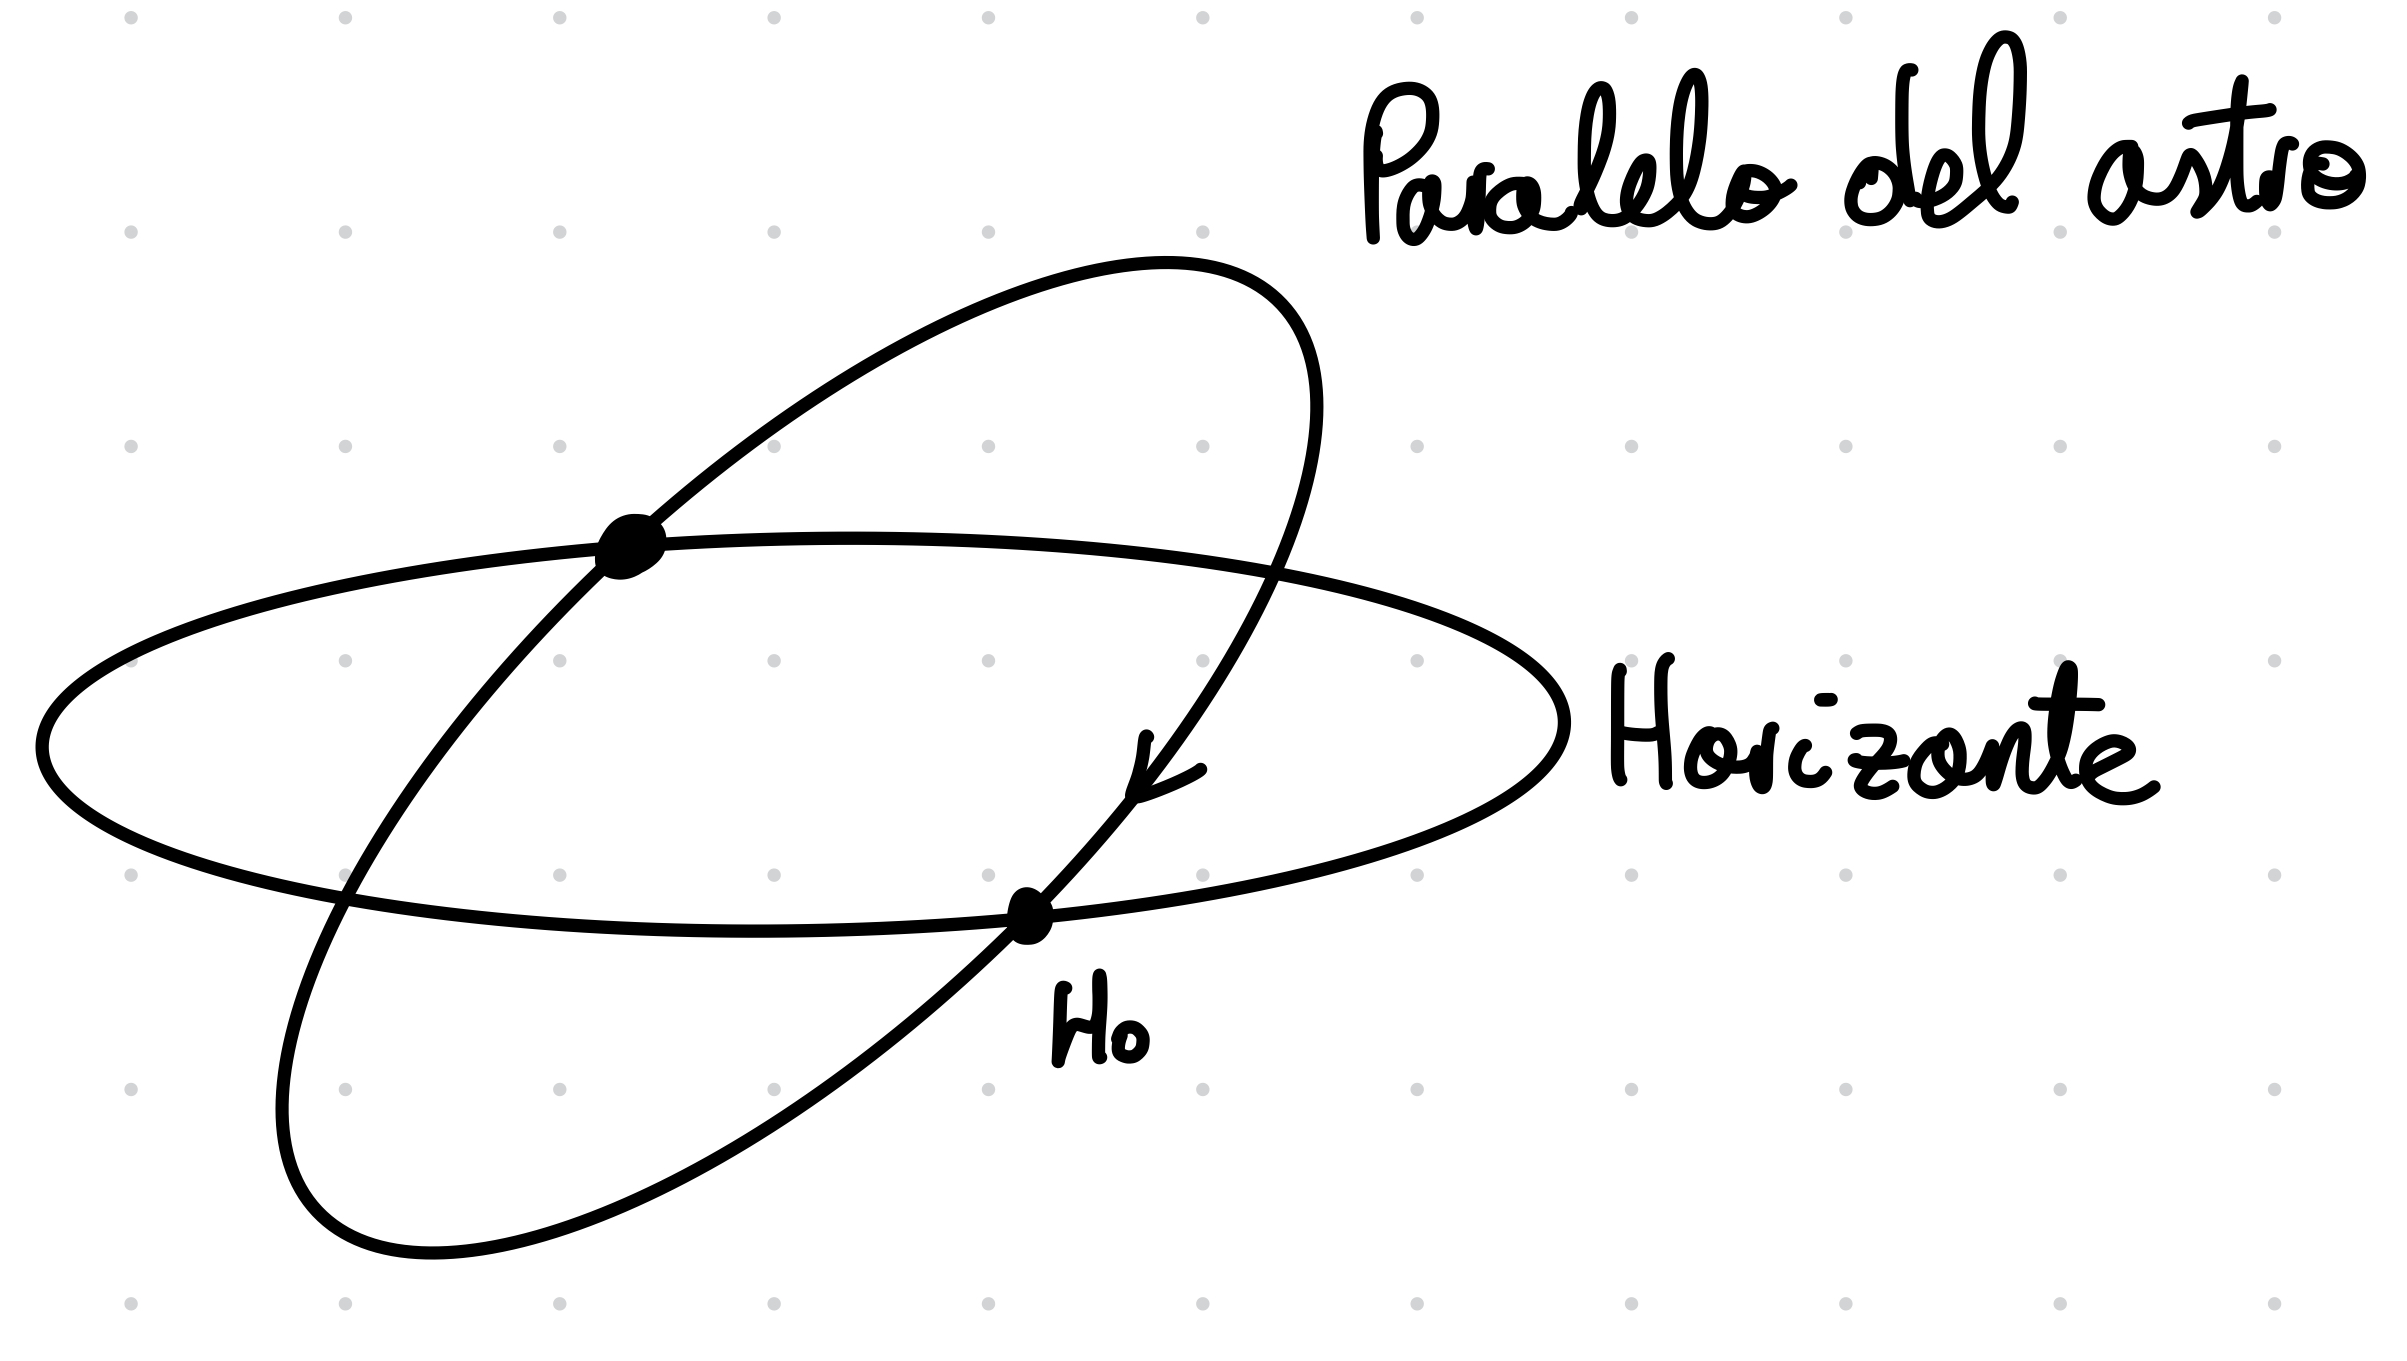
\includegraphics[width=1.0\textwidth]{Cuerpo/Imagenes/01_Ejercicio_2.jpg}
	 \end{minipage}
	 
	 
\end{texercise}

\begin{texercise}
	¿Cuántas horas máximas y mínimas del Sol por encima del horizonte a lo largo de un día podemos tener en Santiago de Compostela? Dato: $\phi=42^\circ,52',40''$.
	 \tcblower
		 
	El máximo de horas ocurre cuando estamos el solsticio de verano. En este caso sabemos que $\delta=\epsilon$. Usando las ecuaicones del primer ejercicio:
		 
	 \begin{equation}
	 	H_0 = 7^h 34^m 57^s \Rightarrow 2H_0 = 15^h 9^m 54^s
	 \end{equation}
	 El mínimo de horas del sol es en el solsticio de invierno.  En este caso
		 
	 \begin{equation}
	 	\delta = - \varepsilon \Rightarrow 2H_0 = 8^h 50^m 4^s
	 \end{equation}
\end{texercise}


\begin{texercise}
	Las coordenadas ecuatoriales absolutas de una estrella son 	$\alpha = 3^{h}45^{m}43^{s}$, y $\delta = 20^\circ8'27''$. ¿Podremos observarla desde la Facultad de Matemáticas ($\phi = 42^\circ52'26''$) en el instante en el que el punto 
	vernal está en la dirección norte? \textbf{[Solución:} Dado que $h < 0^\circ$ 
	($h = -8^\circ24'29''$), la estrella no será visible.\textbf{]}
	\tcblower
	Hola
\end{texercise}
\begin{texercise}
	Un cometa tiene coordenadas ecuatoriales absolutas $\alpha = 10^{h}3^{m}57^{s}$ y $\delta = 8^\circ24'54''$. ¿Cuáles son sus coordenadas eclípticas?  
	\textbf{[Solución:} $\lambda = 150^\circ3'19''$	$\beta = -3^\circ14'31''$.\textbf{]}
	\tcblower
	Hola
\end{texercise}

\tcbstoprecording
